% !TeX spellcheck = it_IT
% !TEX encoding = utf8

\chapter{Galois - Il Genio che non aveva tempo}
\begin{minipage}{1.46\linewidth}
		\begin{flushright}
			\emph{Sfortunatamente non si comprende come i libri scientifici più validi\\ siano quelli in cui l’autore indica chiaramente cosa non sa;\\ un autore fa infatti maggiormente del male ai suoi lettori\\ quando nasconde le difficoltà.}\\
			\vspace{0.5cm}
			\bfseries{Évariste Galois} \\
			\textnormal{(25 Ottobre 1811 – 31 Maggio 1832)}.
		\end{flushright}
\end{minipage}
\section{Évariste Galois - Il profeta}

Rivoluzionario, guerrafondaio, irrispettoso, insofferente verso la mediocrità, passionale e romantico. Del tutto incostante negli studi; geniale, ma refrattario all’istruzione formale e insofferente verso chi non era in grado di seguirlo mentre svolgeva complicati calcoli a mente (inclusi i propri esaminatori). Ancora diciannovenne aveva già risolto un problema che resisteva da secoli agli attacchi dei matematici, ma poiché pochissimi lo avevano capito, era convinto che sarebbe stato dimenticato.

\marginpar{ 
	\captionsetup{type=figure}
	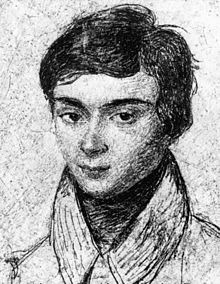
\includegraphics[width=\marginparwidth]{galois}
	\caption[Galois]{Una delle poche immagini di Galois pervenuteci}
	\label{fig:galois}
	}

Eppure la storia oggi gli rende giustizia ricordandolo come uno dei grandi della matematica. Forse il migliore algebrista di sempre. Ma chi era dunque Galois? Perché viene ricordato come l’ultimo matematico romantico?

\section{Una vita appassionata}

1811. L’Impero di Napoleone è all’apogeo. La campagna di Russia è alle porte. Ed è in questo clima che alle porte di Parigi, a Bourg-la-Reine, il 25 ottobre nasce Évariste Galois. Già da giovanissimo mostrò tutti i caratteri dell’énfant prodige. Leggeva e studiava manoscritti dei grandissimi del tempo: Lagrange, Gauss e Abel. Tuttavia mentre i suoi maestri di Matematica lo incoraggiavano e lo seguivano, quelli di tutte le altre materie lo ritenevano tutt’altro che un genio: non si applicava, non eccelleva in nessuna materia che non fosse la matematica e come se ciò non bastasse non si faceva nemmeno problemi a nascondere la sua insofferenza verso le cariche istituzionali che non gli andavano a genio.

Dal padre, sostenitore della Repubblica e sindaco del proprio villaggio nel periodo della Restaurazione, e dallo zio paterno (ufficiale napoleonico) prende la passione politica e comincia ad accostarsi al movimento repubblicano. Tuttavia il suicidio del padre assurdamente provocato per ragioni politiche segnerà profondamente lo spirito del giovane figlio.
\section{Un matematico incompreso}

Galois trascorreva talmente tanto tempo in profondi studi astratti che i suoi contemporanei non lo capivano. Eccone un esempio. Siamo nel 1829. Gaois ha 18 anni. I suoi lavori riguardavano le frazioni continue e la scoperta di nuovi insiemi numerici. Vuole entrare nel più prestigioso istituto di matematica dell’epoca: l’Accademia delle Scienze di Parigi. Presenta come domanda per l’ammissione alcune note sulla risoluzione tramite radicali di equazioni algebriche. Teniamo a mente che gran parte dell’algebra moderna viene da quelle note (se vuoi vedere qualche applicazione delle sue scoperte ecco un nostro recente articolo: I problemi con riga e compasso). I professori del tempo, restii alle idee di un diciottenne e abituati a ben altri calcoli, rifiutano il lavoro. Altri addirittura cestinano le note. Figuratevi come non reagì Galois che non solo si riteneva superiore alla sua commissione giudicatrice ma si mise addirittura a discutere con loro rinfacciandogli di non aver capito la portata delle sue idee.

Dovette a malincuore ripiegare sulla ben meno prestigiosa Scuola Normale.
\section{Il matematico romantico}

Cambiando scuola però i problemi non finirono. Durante i moti del 1830 ha i primi contrasti con le autorità. Ma non si piega. Al contrario, aumenta la propria posizione radicale. Viene prima arrestato, sbattuto in prigione e poi espulso dalla Scuola.

Alexandre Dumas a proposito dell’evento incriminato dell’arresto del giovane scrive:

All’improvviso, nel bel mezzo di una conversazione privata tra me e la persona seduta a sinistra, le mie orecchie sentirono il nome di Luigi Filippo, seguito da cinque o sei fischi. Mi voltai. A quindici o venti posti di distanza da me si stava svolgendo una delle scene più animate della serata. Un giovane che teneva nella stessa mano un bicchiere e un pugnale aperto cercava di farsi sentire dagli altri.
Si trattava di Évariste Galois. Riuscii a percepire solo che si trattava di una minaccia, e che era stato pronunciato il nome di Luigi Filippo. Il coltello aperto lasciava trasparire le intenzioni del giovane.

\section{Uno spirito passionale}

Rilasciato dal carcere nel 1832, si invaghisce di una ragazza. Da qui in poi ci sono ancora molte ombre sulle sua vita ma vi posso raccontare quella che la versione più accreditata racconta.

Lei si chiamava Stephanie Potterin du Motel e Galois l’aveva conosciuta solo pochi mesi prima. La relazione tra i due, però, si era interrotta quasi subito per ragioni che non sono note. Si sa solo che di lì a poco Galois fu sfidato a duello per difendere l’onere della donzella e a sfidarlo fu Ernest Duchatelet, “patriota” e una delle migliori pistole di Francia. E tirarsi indietro non era contemplabile all’epoca.

Oggi possiamo dire con un certo grado di sicurezza che quella di Galois fu probabilmente una congiura: tutto fu organizzato in modo che il giovine si trovasse nel posto giusto al momento sbagliato.

Galois sapeva che quella sarebbe stata la sua ultima notte. Rabbiosamente si rinchiude in casa per raccogliere tutti i suoi lavori e cercare di commentarli in modo che qualcuno possa un giorno riprenderli e fare in modo che le sue idee non vadano perdute. A margine dei fogli si può spesso leggere “non ho tempo… non ho tempo” proprio ad indicare l’ineluttabilità del momento e la pressione che si sentiva addosso… Provate ad immaginare cosa vuol dire avere la completa padronanza di un argomento che attanaglia la mente di matematici illustri da secoli, sapere che da lì a qualche ora la vostra morte si sta avvicinando e non avere il tempo per poter ordinare le vostre idee per evitare che vadano perdute!

Ed è proprio in questa notte che scrive la celebra lettera all’amico Chevalier. Essa è oggi considerata il suo testamento spirituale ai posteri, nonché base della moderna matematica. Nella stessa lettera si pregava Chavalier di far recapitare a Gauss e Jacobi tutti i lavori sulla sua opera di matematico.

“Pregherai pubblicamente Jacobi o Gauss di dare il loro parere, non sulla verità, ma sull’importanza dei teoremi. Dopo questo ci sarà, spero, qualcuno che troverà il suo profitto a decifrare tutto questo guazzabuglio”.

Personalmente, l’ultima volta che ho controllato il profitto si è trovato eccome!

Galois inoltre lascia nella lettera i principali teoremi della futura teoria dei gruppi che porta il suo nome e il legame profondo con la teoria della risoluzione algebrica delle equazioni.

\section{La teoria di Galois}

Prima di concludere però vorrei fare un breve accenno sulla teoria dei gruppi citando un esempio che ho trovato online a questa pagina.\footnote{Matematicamente un \emph{gruppo} è un insieme $ G $ munito di una operazione binaria $ \star $ che ad ogni coppia di elementi $ a,b $ di $ G $ associa un elemento, che indichiamo con $ a \star b $, appartenente a $ G $, rispettando i seguenti assiomi:
	\begin{itemize}
		\item \textbf{proprietà associativa}: dati $ a, b, c\in G $, vale $ (a\star b)\star c = a\star(b\star c) $.
		\item \textbf{esistenza dell'elemento neutro}: esiste in $ G $ un elemento \emph{neutro} $ e $  rispetto all'operazione $ \star $, cioè tale che $ a\star e = e\star a = a $ per ogni $ a\in G $.
		\item \textbf{esistenza dell'inverso}: ad ogni elemento $ a\in G $ è associato un elemento $ a' $, detto inverso di $ a $, tale che $ a\star a'=a'\star a=e $. 
	\end{itemize}
}

Considerate una gara di ciclismo a cui partecipano solo tre corridori. Quanti sono i possibili esiti della gara se i partecipanti non possono tagliare il traguardo contemporaneamente? Se indichiamo i ciclisti con i simboli $ A, B, C $, il problema dei possibili esiti della gara sta allora nel capire in quanti e quali modi si possono mettere in ordine gli oggetti $ A, B, C $.

Un modo efficace di procedere è di mettere in prima posizione, a turno, uno degli elementi e vedere cosa succede dopo, nelle altre posizioni. Per esempio, se il ciclista $ A $ finisce primo, negli altri due posti, cioè in seconda e in terza posizione, possono andare solo gli altri due elementi, e in due soli modi possibili; ripetendo il ragionamento per $ B $ e $ C $ si vede che i modi possibili per ordinarli sono $ 6 $, cioè in matematichese $ 3! = 3\times 2\times 1 =6 $ .

Una sostituzione equivale a operare in un certo modo sugli elementi $ A, B, C $, rispetto a una sostituzione di base (per esempio $ ABC $) presa come riferimento. Allora, la sostituzione $ CBA $ corrisponde al fatto che $ A\to C, B\to B, C\to A $; cioè, in sostanza, al fatto che $ A $ e $ C $ si sono scambiati di posto.

Inoltre, le sostituzioni possono essere anche moltiplicate tra loro, un po’ come si fa con i numeri. Se avete la sostituzione $ CBA $ $ (A\to C, B\to B, C\to A) $ e la sostituzione $ ACB $ $ (A\to A, B \to C, C\to B) $, fare il prodotto tra le due sostituzioni vuole dire applicarle successivamente: si ottiene così $ (A\to C\to B, B\to B\to C, C\to A\to A) $, cioè $ BCA $.

Esiste sempre la sostituzione che lascia inalterato il risultato finale del prodotto, cioè l’elemento neutro (è la sostituzione identica $ ABC, A\to A, B\to B, C\to C $) e la sostituzione che moltiplicata per un’altra dà come risultato la sostituzione identica $ ABC $.
\subsection{Il concetto di Gruppo}

Queste sono alcune delle principali proprietà di ciò che nella matematica moderna va sotto il nome di gruppo. Ossia, l’insieme delle sostituzioni su tre elementi possiede una struttura di gruppo; e il discorso è valido indipendentemente dal numero $ n $ di oggetti considerati.

\marginpar{
	\captionsetup{type=figure}
	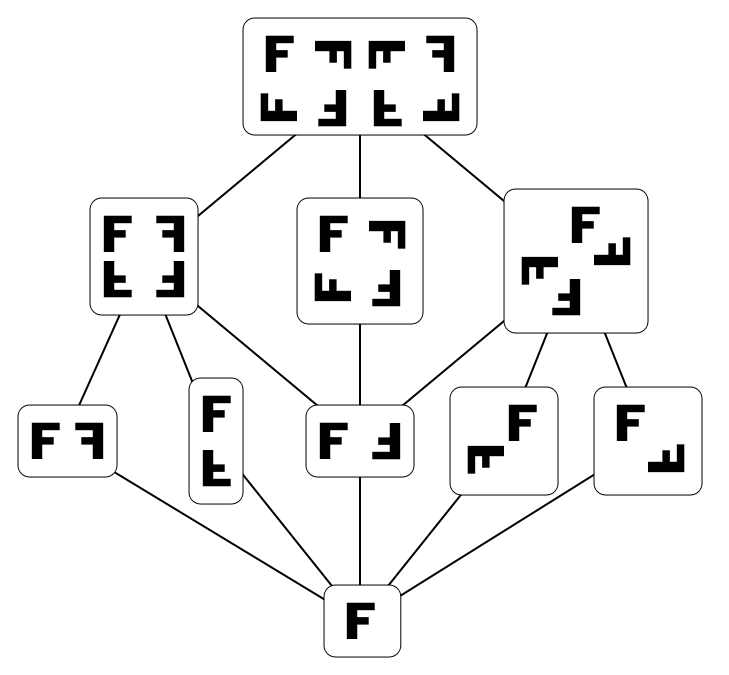
\includegraphics[width=\marginparwidth]{gruppo}
	\caption[Simmetrie del quadrato]{Le simmetrie di un quadrato formano un gruppo di ordine 8. Questo gruppo contiene 1 sottogruppo di ordine 8 (se stesso), 3 sottogruppi di ordine 4, 5 sottogruppi di ordine 2 e 1 sottogruppo di ordine 1 (il sottogruppo \emph{banale}). I sottogruppi sono descritti qui in figura mostrando gli effetti delle singole simmetrie su una figura non simmetrica (la lettera F).}
	\label{fig:gruppo}
}

L’idea di gruppo di sostituzioni è emersa soprattutto in relazione allo studio delle equazioni algebriche, come per esempio l’equazione: $ x^2-2=0 $. In questo caso, si tratta di un’equazione molto semplice da risolvere, ma quando l’equazione è più complessa, in particolare quando è più alto il suo grado, allora il gruppo di sostituzioni permette di risolvere il problema in quella che è ora nota come teoria di Galois.

\section{Il matematico che non aveva tempo}

La mattina del 29 maggio una carrozza viene a prendere Galois. Lo condurrà in una pineta. Non sarà lui il vincitore del duello. A ritrovarlo è un contadino del luogo.

Prima di morire disse al fratello:
”Ho bisogno di tutto il mio coraggio per morire a 20 anni”. 
Il 30 maggio 1832 Évariste Galois muore per traumi subiti allo stomaco da un colpo di arma da fuoco in ospedale. Non aveva nemmeno 20 anni. Viene sepolto in una fossa comune fuori Parigi, dove ancora risiede.

“Mantenete la mia memoria, perché la sorte non mi ha dato abbastanza vita affinché la patria conosca il mio nome”

\medskip

I lavori di Galois rimasero pressoché sconosciuti fino al 1846, quando il matematico francese Joseph Liouville li pubblicò sul suo \emph{Journal de mathématiques pures et appliqueés}, ben 14 anni dopo.

\medskip

Oggi il suo nome è leggenda.
